\section{Analisi dei risultati ottenuti}

%=======================================================================

\begin{frame}{AEAD: ascon128a}

    \begin{center}
        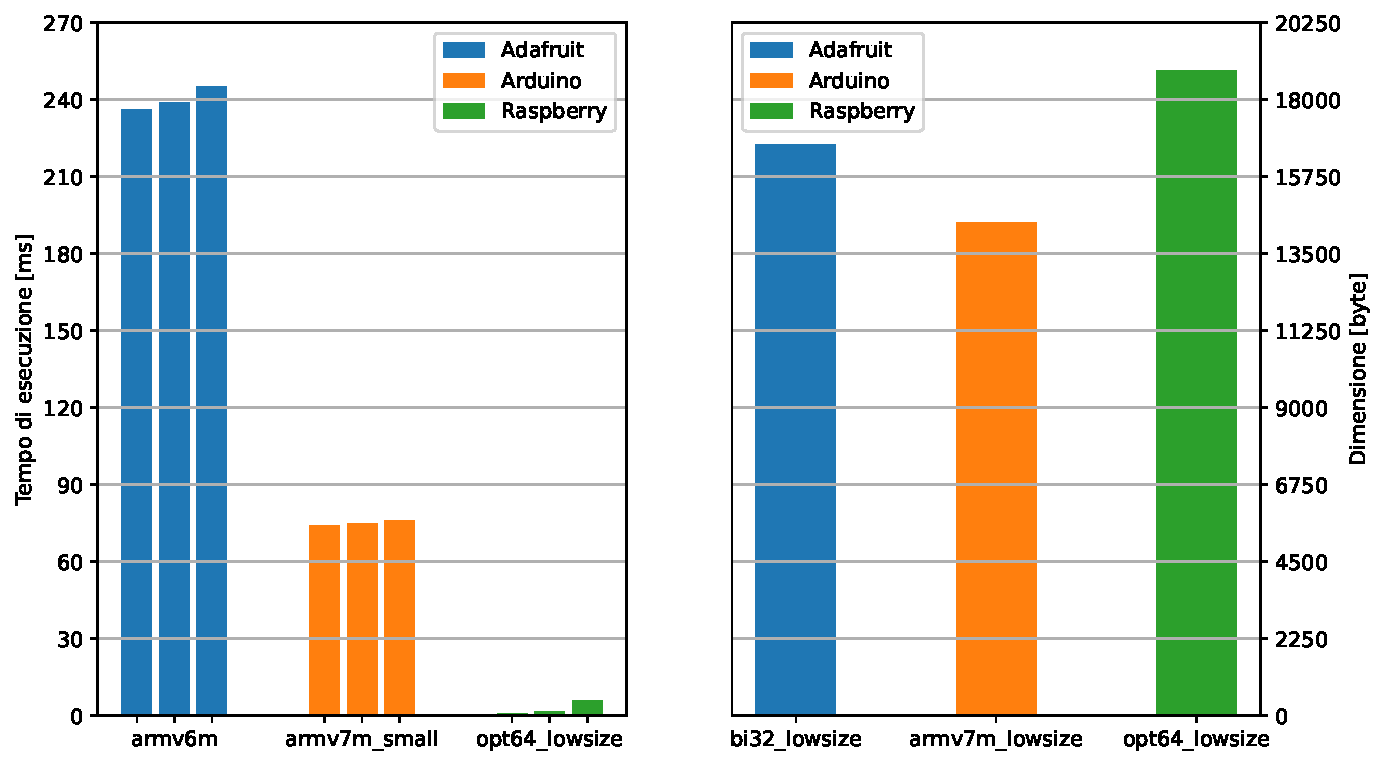
\includegraphics[height=0.40\textwidth]{images/aead.pdf}
    \end{center}
    
\end{frame}

%=======================================================================

\begin{frame}{Hash: asconhasha}

    \begin{center}
        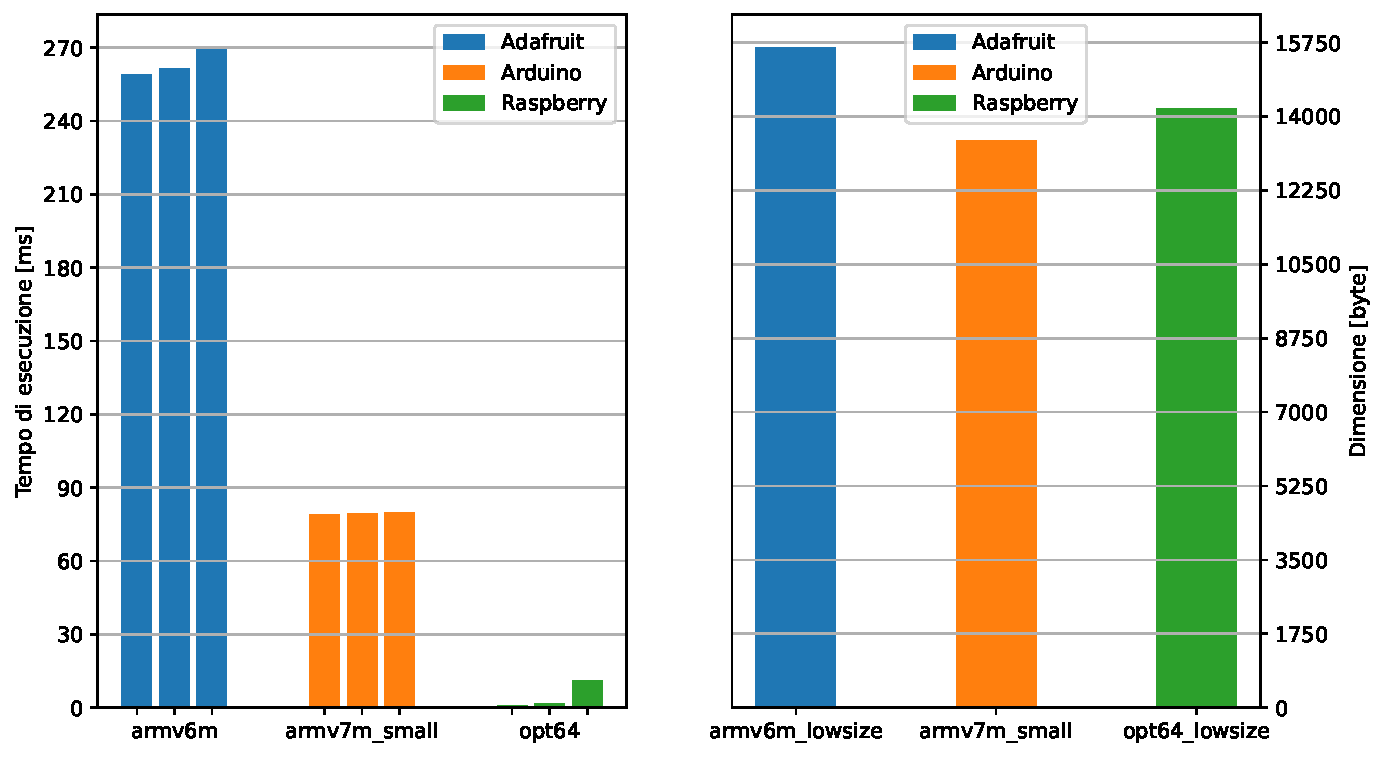
\includegraphics[height=0.40\textwidth]{images/hash.pdf}
    \end{center}
    
\end{frame}

%=======================================================================

\begin{frame}{Auth: asconmaca}

    \begin{center}
        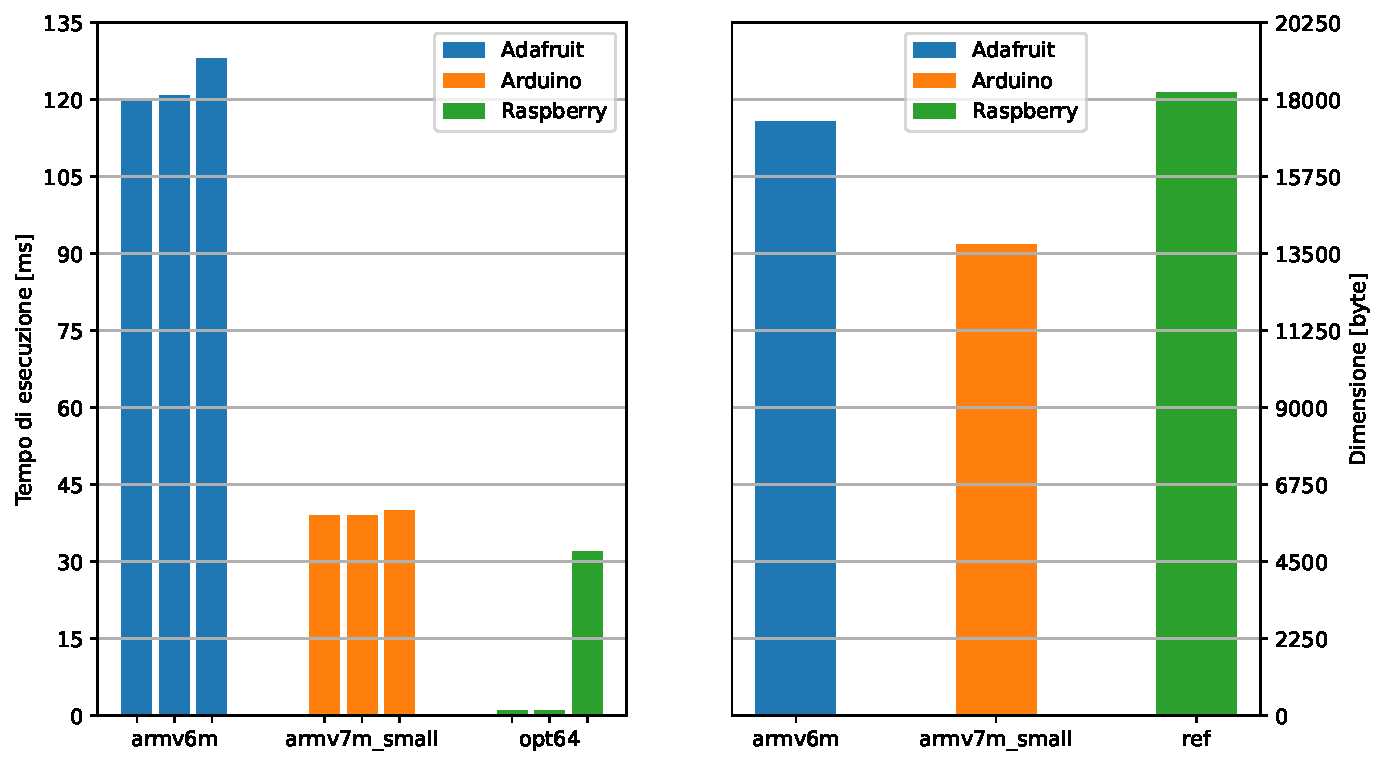
\includegraphics[height=0.40\textwidth]{images/auth.pdf}
    \end{center}
    
\end{frame}

%=======================================================================

\begin{frame}{Migliori implementazioni per ogni dispositivo}

    \begin{table}
        \centering
    	\begin{tabular}{|m{0.20\textwidth}<{\centering}||m{0.20\textwidth}<{\centering}|m{0.20\textwidth}<{\centering}|m{0.20\textwidth}<{\centering}|}
    		\hline
    		\textbf{Dispositivo} & \textbf{Tempo} & \textbf{Spazio} & \textbf{Ibrido} \\
            \hline \hline
            \textbf{Adafruit} & \texttt{armv6m} & \texttt{lowsize} & \texttt{armv6m} \\
            \hline
            \textbf{Arduino} & \texttt{armv7m\_small} & \texttt{armv7m\_small} & \texttt{armv7m\_small} \\
    		\hline
            \textbf{Raspberry} & \texttt{opt64} & \texttt{opt64\_lowsize} & \texttt{opt64} \\
            \hline
        \end{tabular}
    \end{table}

\end{frame}
